% REVISÃO DE LITERATURA-------------------------------------------
\chapter{DISPOSITIVOS LÓGICOS E LÓGICA PROGRAMÁVEL}
\label{cap2}

A lógica programável é um campo que se baseia em princípios e conceitos que permitem a criação de soluções de hardware por meio do uso de dispositivos programáveis. Esses dispositivos são capazes de executar funções lógicas específicas, as quais podem ser definidas pelo fabricante ou pelo usuário, utilizando tanto software quanto hardware.
Além disso, a lógica programável tem sido amplamente utilizada em diversos campos, como em sistemas embarcados \cite{mishra2018fpga}, comunicações digitais \cite{proakis2006digital}, processamento de sinais \cite{shynk1999review}, entre outros. Esses avanços têm sido possíveis graças aos esforços contínuos de pesquisa e desenvolvimento em hardware e software. De acordo com \citeonline{brown2013field}, os dispositivos programáveis podem ser classificados em várias categorias, dependendo do nível de abstração e da tecnologia utilizada. 

\section{Introdução aos Dispositivos Lógicos Programáveis}

Na década de 1970, surgiram no mercado os dispositivos lógicos programáveis (PLD), que revolucionaram a área de circuitos lógicos combinacionais. Um PLD é basicamente um tipo de chip para uso geral que possui hardware configurável e/ou reconfigurável, em contraste com os microprocessadores, que executam programas por meio de hardware fixo \cite{pedroni2010eletronica}. Dentro da categoria de PLDs, há uma ampla variedade de chips disponíveis, sendo a maioria deles agrupados sob o termo Dispositivos Lógicos Programáveis Simples (SPLD). No entanto, os mais relevantes e conhecidos são os Dispositivos Lógicos Programáveis Complexos (CPLD), os Arranjos de Portas Programáveis em Campo (FPGA) e os Circuitos Integrados de Aplicação Específica (ASIC) \cite{moore2017fpgas}. 

\subsection{SPLD e CPLD}
Geralmente, um SPLD é utilizado em aplicações que exigem menos complexidade, como projetos de pequeno porte. Existem vários tipos de SPLDs disponíveis no mercado, incluindo PALs (\textit{Programmable Array Logic}) e GALs (\textit{Generic Array Logic}). Cada um desses tipos tem suas próprias características e vantagens, tornando-os adequados para diferentes aplicações \cite{floyd2009sistemas}. Já o CPLD é um dispositivo eletrônico programável que permite a criação de circuitos lógicos complexos em um único componente. Eles são compostos por vários SPLDs interconectados por meio de um arranjo complexo e programável. A Figura \ref{fig:Arqui_CPLD} ilustra a estrutura de um CPLD convencional \cite{pedroni2010eletronica}. Essa estrutura possibilita uma maior capacidade para projetar circuitos lógicos maiores e mais complexos do que os que poderiam ser criados com apenas um SPLD.

\begin{figure}[!htb]
    \centering
    \caption{Arquitetura básica de CPLDs}
    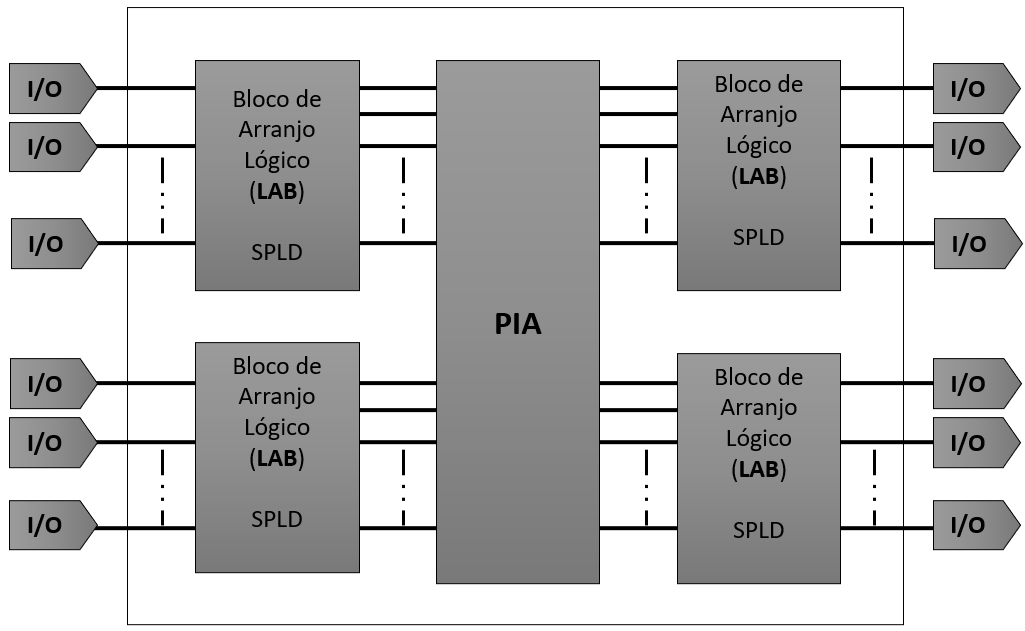
\includegraphics[scale=0.5]{figuras/ARQ_CPLD2.png}\\
    {\footnotesize Fonte: Adaptado de \cite{floyd2009sistemas}.}
    \label{fig:Arqui_CPLD}
\end{figure}

O CPLD pode ser reprogramado a qualquer momento, permitindo que o circuito seja atualizado e adaptado às necessidades do projeto. Cada arranjo SPLD em um CPLD é chamado de Bloco de Arranjo Lógico (LAB), que é uma unidade lógica programável que pode executar funções lógicas complexas. Cada LAB é interconectado por linhas de interconexão programáveis, chamadas de Arranjo de Interconexões Programáveis (PIA). Essas interconexões programáveis permitem que os blocos lógicos se comuniquem entre si e formem circuitos digitais complexos e customizados \cite{floyd2009sistemas}. 

Com esta classe de PLD, é possível implementar funções digitais de média e alta complexidade, incluindo sistemas sequenciais e combinacionais, como registradores de deslocamento, contadores, multiplexadores e decodificadores. Além disso, eles são frequentemente utilizados em aplicações de alta velocidade, como em sistemas de processamento de sinais digitais, processamento de imagens e em sistemas de controle de automação industrial \cite{pedroni2010eletronica} .

\subsection{FPGA}
Um FPGA, em tradução, um Arranjo de Portas Programáveis em Campo, é um dispositivo lógico que possui uma estrutura interna ainda mais complexa que um CPLD. \citeonline{ordonez2003projeto} afirma que a estrutura fundamental de um FPGA pode variar entre fabricantes, famílias de dispositivos e até mesmo dentro de uma mesma família, mas existem alguns elementos essenciais que são mantidos, como é mostrado na Figura \ref{fig:fpga_01}, os três elementos básicos que constituem um FPGA são :

\begin{enumerate}[label={\noNalph{enumi})}]
    \item CLB (\textit{Configurable Logic Block}): Blocos Lógicos Configuráveis, unidade lógica de um FPGA; 
    \item SB (\textit{Switch Box}): Caixa de Conexão, responsável pela conexão entre os CLBs,  através de canais de roteamento;
    \item IOB (\textit{In/Out Block}): Blocos de Entrada/Saída, responsáveis pela interface com o ambiente.
\end{enumerate}


\begin{figure}[!htb]
    \centering
    \caption{Representação dos elementos básicos de um FPGA}
    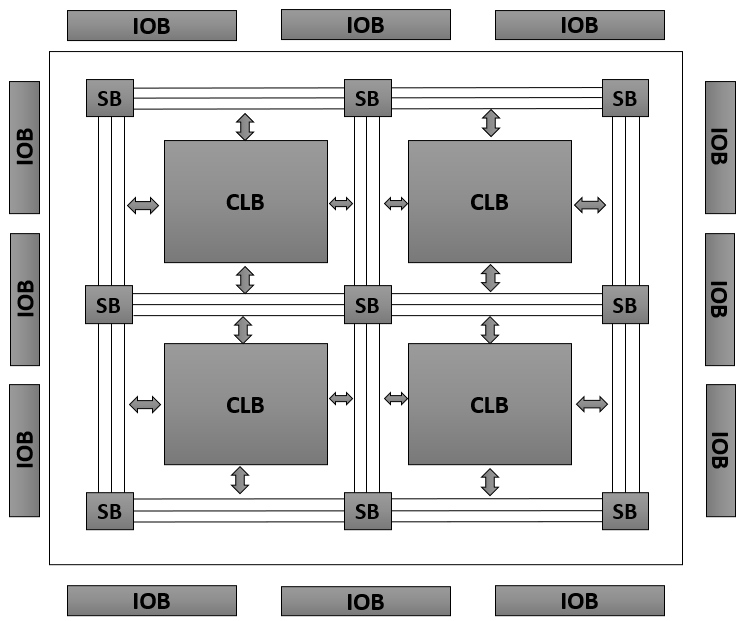
\includegraphics[height = 9cm]{figuras/fpga_2.png}\\
    {\footnotesize Fonte: Adaptado de \cite{floyd2009sistemas}}
    \label{fig:fpga_01}
\end{figure}

A característica programável em um FPGA é semelhante à interconexão de chaves em uma placa de prototipagem que pode ser alterada pelo projetista. No FPGA, essa interconexão pode ser reprogramada pelo usuário ou pelo designer no laboratório ou em campo. Isso é possível porque o FPGA é composto por uma matriz de células lógicas, que podem ser programadas para executar funções específicas, como portas lógicas, registradores, memórias, entre outras. A programação é feita através de um processo de configuração que pode ser realizado sem a necessidade de retirar o dispositivo do circuito, o que significa que é possível atualizar ou reconfigurar o FPGA sem ter que substituir o hardware \cite{roth2004circuit}. Por isso, essa matriz de portas lógicas (\textit{Gate Array}) é chamada de programável em campo (\textit{Field Programmable}). Os tipos de portas lógicas programáveis incluem todas as portas básicas para atender a qualquer necessidade \cite{SmithFranzon08}. 

\subsubsection{Blocos Lógicos Configuráveis (CLB)}

Os blocos lógicos configuráveis são uma das principais unidades funcionais dos FPGA. Cada CLB consiste em uma rede de células lógicas com a lógica desejada, além de possuir uma variedade de elementos de armazenamento, tais como flip-flops, latches e registradores. A arquitetura interna dos CLBs varia entre os fabricantes de FPGA, mas em geral eles possuem recursos de roteamento programáveis que permitem a interconexão entre os CLBs e outros blocos funcionais do FPGA. A figura \ref{fig:clb_bloc} ilustra a disposição dos CLBs essenciais nas interconexões programáveis globais em linha/coluna. Essas interconexões têm a função de estabelecer as conexões necessárias para interligar os blocos lógicos entre si. \cite{roth2004circuit}.

Os CLBs possuem grande flexibilidade, permitindo que os designers de hardware personalizem a lógica interna de acordo com as necessidades de seus projetos. Isso é possível através da programação do FPGA por meio de linguagens de descrição de hardware (HDL), como o VHDL, que permite a descrição da lógica desejada em um nível de abstração alto e
portável entre diferentes fabricantes de FPGA \cite{silva2013introducao}.

\begin{figure}[!ht]
    \centering
    \caption{Blocos lógicos configuráveis básicos (CLBs) dentro de interconexões programáveis globais em linha/coluna.}
    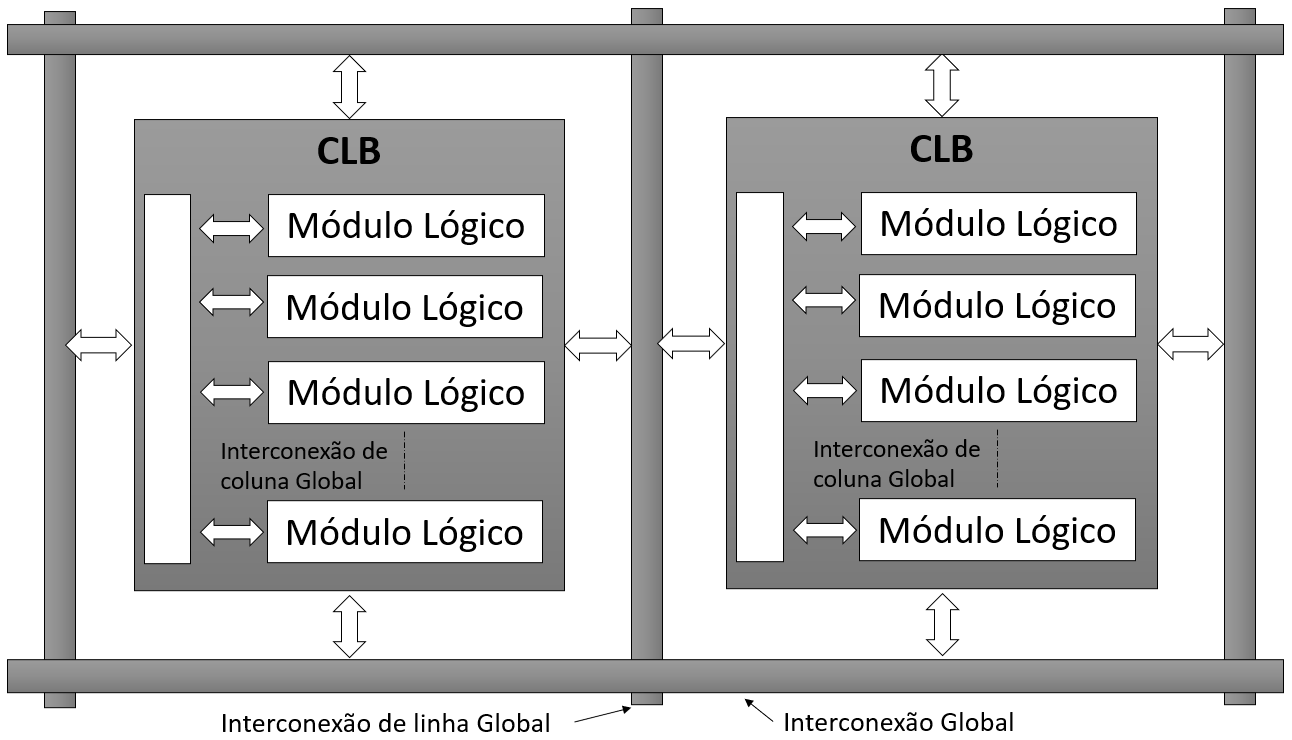
\includegraphics[height = 7.5cm]{figuras/clb_bloc0.png}\\
    {\footnotesize Fonte: Adaptado de \cite{floyd2009sistemas}}
    \label{fig:clb_bloc}
\end{figure}

Cada CLB em um FPGA é composto por vários módulos lógicos menores e uma interconexão programável local que permite a conexão entre esses módulos dentro do CLB. Esses módulos lógicos podem ser configurados como lógica combinacional, lógica registrada ou uma combinação de ambas. A Figura \ref{fig:mod_log} ilustra o diagrama em bloco de um módulo lógico típico baseado em LUT (\textit{Look Up Table}). Uma LUT, ou tabela de busca, é uma forma de memória programável utilizada para gerar funções lógicas combinacionais em formato de soma-de-produtos \cite{floyd2009sistemas}.

\begin{figure}[!ht]
    \centering
    \caption{Modulo Lógico.}
   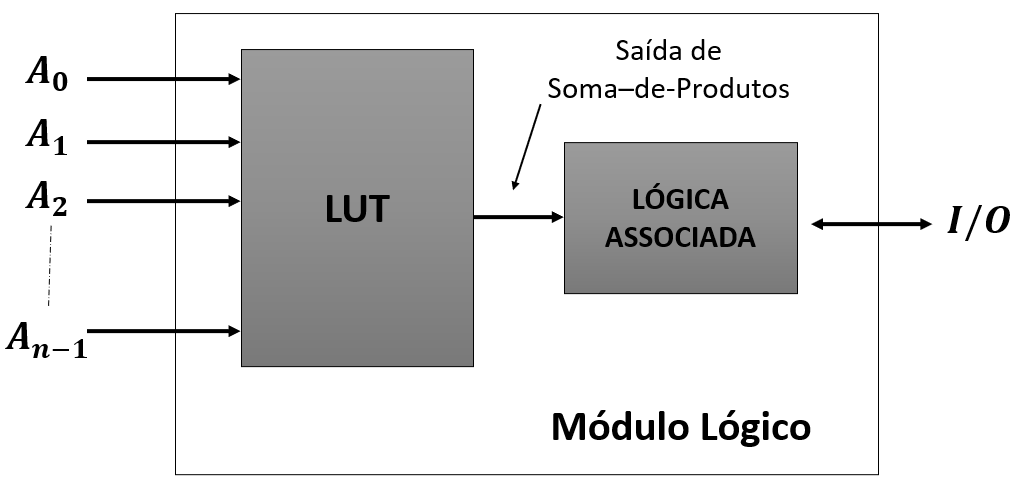
\includegraphics[height = 5.5cm]{figuras/Mod_log.png}\\
    {\footnotesize Fonte: Adaptado de \cite{floyd2009sistemas}}
    \label{fig:mod_log}
\end{figure}

\subsubsection{Caixa de Conexões (SB)}

As Caixas de Conexões servem para unir as interconexões programáveis, sendo estas responsáveis por estabelecer a conexão entre os CLBs e os blocos de entrada/saída (IOB) para implementar a lógica digital desejada. Essas interconexões são constituídas por um conjunto de elementos programáveis, como chaves, multiplexadores e buffers, que permitem a configuração do caminho de sinal entre os blocos
\cite{brown1992field}.

Além disso, a disposição das interconexões também é importante para o desempenho e eficiência do FPGA. Por exemplo, a utilização de canais de roteamento que permitem a
comunicação vertical e horizontal entre os CLBs, além de reduzir a latência e minimizar a interferência entre os sinais, também possibilita a implementação de circuitos mais complexos \cite{wong2007introduction}.

\subsubsection{Blocos de Entrada e Saída (IOB)}

Os blocos de entrada e saída são responsáveis por fornecer uma interface entre o circuito digital do FPGA e o mundo externo. Eles permitem com que haja a comunicação entre dispositivos, como sensores, atuadores, processadores e outros circuitos digitais.Estes são projetados para serem configuráveis e suportar vários padrões de comunicação, como interfaces seriais, paralelas e diferencias, entre outras. Eles são compostos por circuitos específicos, como registradores, buffers, multiplexadores e transceptores, que são configuráveis para atender às necessidades do projeto \cite{brown2013field, maxfield2004design}.

A organização dos blocos de entrada e saída varia de acordo com a arquitetura do dispositivo e a família do FPGA. Por exemplo, alguns FPGA possuem blocos de entrada e saída dedicados que são alocados em áreas específicas do dispositivo, enquanto outros possuem blocos de entrada e saída espalhados por toda a matriz de lógica do dispositivo \cite{xilinx2021ultrascale}.

\section{Linguagem de Descrição de Hardware - HDL}

Dispositivos lógicos programáveis, como os FPGAs, requerem o uso de uma linguagem específica para implementar circuitos físicos em seu próprio hardware. Essa linguagem é conhecida como Linguagem de Descrição de Hardware (HDL) \cite{ordonez2003projeto}.

As HDLs são estruturadas de forma a permitir a descrição abstrata do comportamento de hardwares, possibilitando a modelagem e representação da estrutura e funcionamento de circuitos em diferentes níveis de abstração durante o processo de projeto \cite{ordonez2003projeto}. Isso oferece aos projetistas maior flexibilidade na descrição de circuitos complexos. Anteriormente, essas linguagens eram comumente empregadas para a verificação de lógica. No entanto, com o surgimento dos algoritmos de síntese lógica, tornou-se viável descrever o fluxo de dados dos circuitos em níveis de transferência de registradores (RTL), simplificando a descrição de circuitos digitais. Com isso, detalhes como portas lógicas e interconexões passaram a ser processados automaticamente pelos algoritmos de síntese lógica. \cite{costa2014desenvolvimento}. 

As linguagens de descrição de hardware oferecem várias vantagens em relação aos projetos tradicionais baseados em esquemas elétricos. Permitem a descrição de circuitos digitais de forma independente da tecnologia de fabricação, graças ao nível de abstração dessas linguagens. Além disso, permitem a verificação funcional dos circuitos em estágios iniciais do projeto e facilitam a análise de falhas e erros, uma vez que as HDLs são linguagens textuais semelhantes às linguagens de programação convencionais, como C, C++, Java, entre outras \cite{costa2014desenvolvimento}. 

Existem várias HDLs disponíveis, porém, as mais conhecidas e amplamente utilizadas são a linguagem Verilog e a linguagem VHDL (VHSIC \textit{Hardware Description Language,} onde VHSIC - \textit{Very High Speed Integrated Circuit}) \cite{ordonez2003projeto}.


\subsection{Conceitos Fundamentais do VHDL}

A linguagem VHDL é baseada em uma estrutura hierárquica, onde os componentes são definidos em níveis de abstração, desde o nível mais alto até o nível mais baixo. Isso permite a criação de modelos complexos, divididos em blocos menores e interconectados. No VHDL, a estrutura básica de um design é composta por entidades e arquiteturas (Figura \ref{fig:vhdl_blocos}). A entidade descreve a interface do componente, definindo as portas de entrada e saída, bem como quaisquer parâmetros genéricos. A arquitetura, por sua vez, contém a descrição do comportamento interno do componente, especificando as operações lógicas e a lógica de controle \cite{harris2015digital}. Dentro desses blocos do design, um circuito lógico ou função pode ser facilmente descrito \cite{sousa2017projeto}. Um design em VHDL começa com um bloco de bibliotecas e pacotes, que fornecem funções uteis ao projeto proposto, seguindo para o bloco de entidade que descreve a interface para o design.

\begin{figure}[!htb]
    \centering
    \caption{Estrutura da programação VHDL em blocos}
    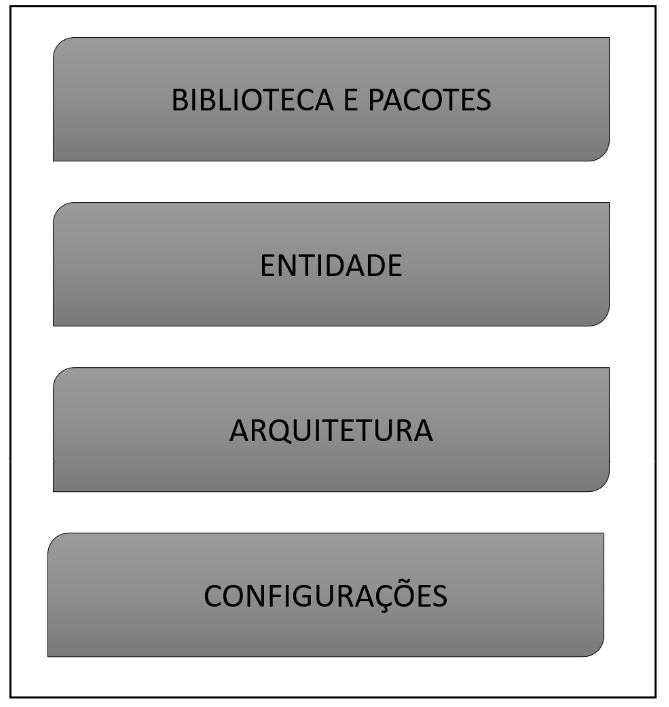
\includegraphics[scale=0.37]{figuras/ESTR_VHDL.png}\\
    {\footnotesize Fonte: Autoria própria.}
    \label{fig:vhdl_blocos}
\end{figure}

A interface define os sinais lógicos de entrada e saída do circuito projetado. O bloco de arquitetura descreve a operação interna do design. Dentro desses blocos, existem vários outros blocos funcionais usados para construir os elementos de design do circuito lógico sendo criado. Após a criação do projeto, ele pode ser simulado e sintetizado para verificar seu funcionamento lógico \cite{ordonez2003projeto}. A estrutura de uma descrição VHDL é mostrado na figura \ref{fig:vhdl_blocos_estrut}.

\begin{figure}[!htb]
    \centering
    \caption{A estrutura de uma descrição VHDL com os seus blocos}
    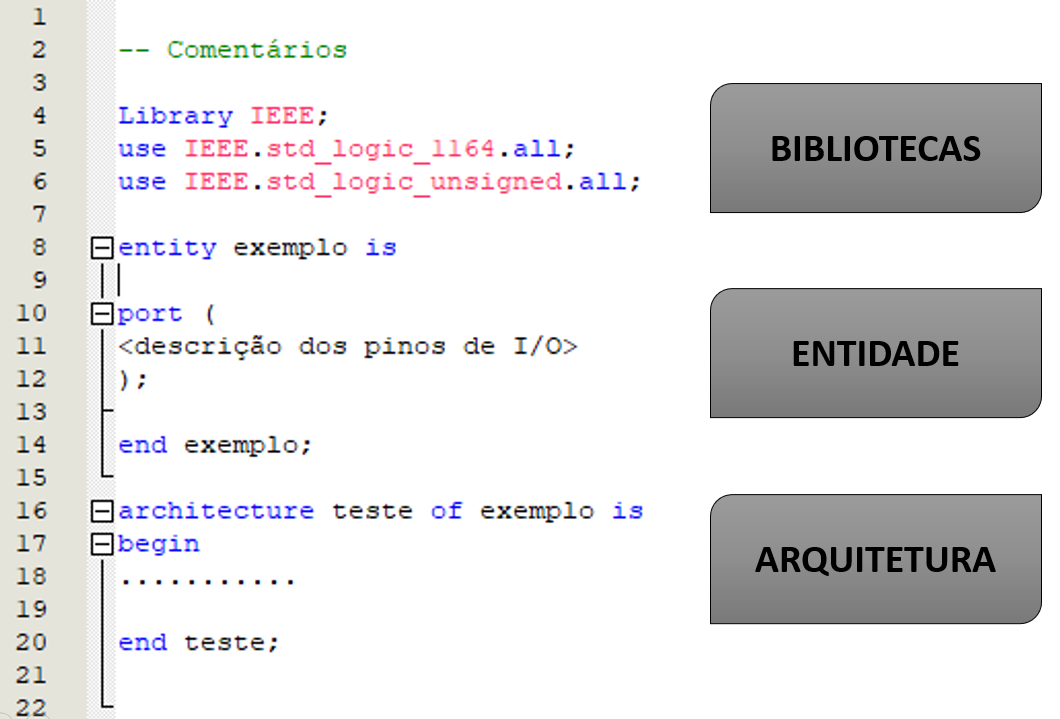
\includegraphics[height = 9cm]{figuras/estrut_blocVHDL.png}\\
    {\footnotesize Fonte: Autoria própria.}
    \label{fig:vhdl_blocos_estrut}
\end{figure}
 
\subsubsection{Declaração de biblioteca e Pacotes}

As bibliotecas e os pacotes são conjuntos de declarações usadas para um determinado fim. Pode ser um conjunto de subprogramas, ou funções que operem com um tipo de dado, assim como pode ser um conjunto de declarações necessárias para modelar um determinado projeto. Uma biblioteca é usada para organizar e gerenciar diferentes unidades de design em um projeto VHDL. É comum criar diferentes bibliotecas para organizar e armazenar unidades de design relacionadas. Por exemplo, uma biblioteca pode ser criada para armazenar unidades de design relacionadas a interface serial, enquanto outra biblioteca pode ser criada para armazenar unidades de design relacionadas a processamento de sinais \cite{roth2004circuit}.

Os pacotes são usados para definir e compartilhar constantes, tipos de dados, funções, procedimentos e outras construções que podem ser usadas em várias unidades de design. Os pacotes podem ser usados para evitar a repetição de código e facilitar a reutilização de código em diferentes unidades de design \cite{ordonez2003projeto}. Por exemplo, um pacote pode ser criado para definir um tipo de dado personalizado que é usado em várias unidades de design. 
Bibliotecas e Pacotes mais utilizados estão citados no quadro \ref{quadro_1}.
%+++++++++++++++++++++++++++++++++++++++++++++++

\begin{quadro}[h]
    \caption{Pacotes mais utilizados (Biblioteca IEEE)}
    \label{quadro_1}
    \centering
     \begin{tabular}{|c|p{3cm}|p{8cm}|}
      \hline
      \textbf{Pacote} & \textbf{Tipos de dados} & \textbf{Descrição} \\
      \hline
      std\_logic & std\_logic e std\_logic\_vector & Define o padrão para descrever a interconexão entre tipos de dados usados na linguagem VHDL \\
      \hline
       std\_logic\_arith & Especifica tipos de dados sinalizados e não sinalizados & Funções de conversão, operações aritméticas e comparações para uso de dados sinalizados e não sinalizados \\
      \hline
       std\_logic\_unsigned & std\_logic\_vector & Define funções que permitem usar tipos de dados std\_logic\_vector, como se fossem tipo de dado não sinalizado \\
      \hline
       std\_logic\_signed & std\_logic\_vector & Define funções que permitem usar tipos de dados std\_logic\_vector, como se fossem tipo de dado sinalizado \\
      \hline
       numeric\_std & & Substitui os pacotes usados juntos std\_logic\_atith, std\_logic\_unsigned e std\_logic\_signed \\
      \hline                 
    \end{tabular}
  \vspace{1.5pt}
  \caption*{\footnotesize Fonte: \cite{ordonez2003projeto}}
\end{quadro}

A declaração do uso de pacotes e bibliotecas é mostrada no quadro \ref{quadro_2}. O uso de .all implica que todos os elementos da biblioteca podem ser usados.

\subsubsection{Declaração de Entidade}

Modelo de tabela:

\begin{table}[htb]
\ABNTEXfontereduzida
\center \caption{Parâmetros da Condutividade Intrabanda do Grafeno \cite{b5}\cite{b13}}
\label{Tab}
\begin{tabular}{p{0.6cm} p{2cm} p{2cm} p{6cm}}
  \hline
   \textbf{ } & \textbf{Valor}  & \textbf{Unidade}  & \textbf{Descrição}  \\[1.5pt]
   	\hline
$e$  &  $1,60\times10^{-19}$  &   $C$  &    Carga do Elétron\\[1.5pt]
$\hbar$   &   $1,05\times10^{-34}$ & $J\!\cdot\!s/rad $ & Constante de Plank Reduzida\\[1.5pt]
$k_B$   &   $1,38\times10^{-23}$ & $J/K $ & Constante de Boltzmanm\\[1.5pt]
$T$   &   $300$ & $K$ &  Temperatura\\
$\sigma_0$   &   $e^2/4\hbar$ & $S\!\cdot\!rad$ & Condutividade HF\\[1.5pt]
$\mu_c$   &   $0; 0,25; 0,5$ & $eV$ & Potencial Químico\\[1.5pt]
$\tau$   &   $0,5$ & $ps$ & Tempo de Amortecimento\\[1.5pt]
\hline
\end{tabular}  
  \vspace{1.5pt}
  \caption*{\footnotesize Fonte: \cite{ordonez2003projeto}}
\end{table}

Primeiramente, para modo TE ( Fig. \ref{Fig9}a), os campos elétrico e magnético no meio 1 são compostos pela onda incidente e pela onda refletida, de forma que:
\begin{equation}\label{eq3.2}
\textbf{E}_1(x,z) = -\hat{a}_y\left[E_{iy}e^{-jk_{z1}(z+d_1)} + E_{ry}e^{+jk_{z1}(z+d_1)}\right]e^{-jk_x x}  
\end{equation}
\begin{equation}\label{eq3.3}
\begin{split}
\textbf{H}_1(x,z) = \hat{a}_x\left[H_{ix}e^{-jk_{z1}(z+d_1)} - H_{rx}e^{+jk_{z1}(z+d_1)}\right]e^{-jk_x x} \qquad\qquad
\\
-\hat{a}_z\left[H_{iz}e^{-jk_{z1}(z+d_1)} + H_{rz}e^{+jk_{z1}(z+d_1)}\right]e^{-jk_x x} 
\end{split}
\end{equation}

\noindent onde $E_{iy}$, $H_{ix}$ e $H_{iz}$ são as amplitudes dos campos EH que compõem a onda incidente, e $E_{ry}$, $H_{rx}$ e $H_{rz}$ são as amplitudes dos campos EH que compõem a onda refletida.
\begin{equation}\label{eq3.2}
\textbf{E}_1(x,z) = -\hat{a}_y\left[E_{iy}e^{-jk_{z1}(z+d_1)} + E_{ry}e^{+jk_{z1}(z+d_1)}\right]e^{-jk_x x}  
\end{equation}